%% LyX 2.2.2 created this file.  For more info, see http://www.lyx.org/.
%% Do not edit unless you really know what you are doing.
% \documentclass[sigconf, english]{acmart}
\documentclass[english]{sig-alternate}
% \usepackage{fouriernc,amsmath}
\usepackage[T1]{fontenc}
\usepackage[latin9]{inputenc}
\usepackage{color}
\definecolor{note_fontcolor}{rgb}{0.800781, 0.800781, 0.800781}
\usepackage{verbatim}
\usepackage{float}
\usepackage{amsmath}
% \usepackage{amsthm}
\usepackage{graphicx}

\makeatletter

%%%%%%%%%%%%%%%%%%%%%%%%%%%%%% LyX specific LaTeX commands.
%% The greyedout annotation environment
\newenvironment{lyxgreyedout}
  {\textcolor{note_fontcolor}\bgroup\ignorespaces}
  {\ignorespacesafterend\egroup}
%% A simple dot to overcome graphicx limitations
\newcommand{\lyxdot}{.}

\floatstyle{ruled}
\newfloat{algorithm}{tbp}{loa}
\providecommand{\algorithmname}{Algorithm}
\floatname{algorithm}{\protect\algorithmname}

%%%%%%%%%%%%%%%%%%%%%%%%%%%%%% Textclass specific LaTeX commands.

% \newtheorem{thm}{\protect\theoremname}

%%%%%%%%%%%%%%%%%%%%%%%%%%%%%% User specified LaTeX commands.
% \documentclass[english]{sig-alternate-05-2015}
\usepackage{calc}
%\usepackage{amsthm}
\usepackage{verbatim}


%% without following commands, amsthm complains proof being already defined 
\let\proof\relax
\let\endproof\relax
\usepackage{amsthm}
\theoremstyle{plain}

\usepackage{graphicx}


\usepackage{mdwlist}% compact lists

\usepackage{relsize}% relative font sizes
\usepackage{todonotes}% private notes
\usepackage{breqn}


\usepackage{soul}


\usepackage{color}


% \usepackage{hyperref}
\PassOptionsToPackage{pdfpagelabels=false}{hyperref} 
% \hypersetup{bookmarks=true,bookmarksnumbered=true,pdfstartview=FitB,colorlinks=true,pdfborder=0 0 0}



% \usepackage{xspace}

% \usepackage[sort&compress]{natbib}

\usepackage{comment}






%% for manually breaking cells in tables.
\newcommand{\specialcell}[2][c]{%
  \begin{tabular}[#1]{@{}l@{}}#2\end{tabular}}


%%%%%%%%%%%%%%%%%%%%%%%%%%%%%% LyX specific LaTeX commands.
%% Because html converters don't know tabularnewline
\providecommand{\tabularnewline}{\\}


%%%%
\usepackage{booktabs}
\newcommand{\ra}[1]{\renewcommand{\arraystretch}{#1}}

\usepackage[nameinlink,capitalize,noabbrev]{cleveref}
%%%%%%%%%%%%%%%%%%%%%%%%%%%%%% Textclass specific LaTeX commands.
\theoremstyle{plain}
\newtheorem{thm}{\protect\theoremname}\theoremstyle{definition}
\newtheorem{defn}{\protect\definitionname}
\crefname{thm}{Theorem}{Theorems}
\crefname{defn}{Definition}{Definitions}
%%%%%%%%%%%%%%%%%%%%%%%%%%%%%% User specified LaTeX commands.
\usepackage{algorithm}



% \usepackage{algpseudocode}
\usepackage[noend]{algpseudocode}%to remove endif, and endfors from pseudocode




\usepackage{babel}
\providecommand{\definitionname}{Definition}
\providecommand{\theoremname}{Theorem}
\usepackage{balance}

\newcommand{\bigo}[1]{\ensuremath{\mathcal{O} \left ( #1 \right )}}
\newcommand{\async}{\textsc{Async}}
% \usepackage[noabbrev]{cleveref}

%========== Custom typographic commands ==========
\newcommand{\emailAddr}[1]{\texttt{\smaller {#1}}}
\newcommand{\mailtoLink}[2]{\href{mailto:#2}{\emailAddr{#1}}}
\newcommand{\refSection}[1]{Section~\ref{#1}}
\newcommand{\refsec}[1]{\S~\ref{#1}}
\newcommand{\refequ}[1]{eq.~\eqref{#1}}
\newcommand{\refEquation}[1]{Equation~\eqref{#1}}
\newcommand{\refFigure}[1]{Figure~\ref{#1}}
\newcommand{\reffig}[1]{fig.~\ref{#1}}
\newcommand{\refDefinition}[1]{Definition~\ref{#1}}
\newcommand{\refdef}[1]{defn.~\ref{#1}}
\newcommand{\refAlgorithm}[1]{Algorithm~\ref{#1}}
\newcommand{\refalg}[1]{alg.~\ref{#1}}
\newcommand{\refAlg}[1]{Alg.~\ref{#1}}
\newcommand{\refTable}[1]{Table~\ref{#1}}
\newcommand{\reftab}[1]{table~\ref{#1}}
\newcommand{\refTheorem}[1]{Theorem~\ref{#1}}
\newcommand{\refthm}[1]{thm.~\ref{#1}}
\newcommand{\refprep}[1]{prepostion~\ref{#1}}
\newcommand{\ramki}[1]{{\color{red}{\bf [Ramki: #1]}}}


\newcounter{todocounter}
\newcommand{\TODO}[1]{{\color{red}\textbf{\refstepcounter{todocounter}  \arabic{todocounter}. #1}}}
%========== Document Specific commands ==========

\setlength{\textfloatsep}{0pt}% Remove \textfloatsep
\newcommand{\etal}{\textit{et al}.}

\newcommand{\sv}{LP}
\newcommand{\asynclp}{asynchronous-\sv}
\newcommand{\synclp}{synchronous-\sv}
\newcommand{\ftsv}{\textsc{FT-LP}}
\newcommand{\graphname}[1]{\emph{#1}}

\newcommand{\CCVAL}{$CC$}
\newcommand{\icomment}[1]{\textbf{ \textcolor{red} {#1}}}
\newtheorem{prop}{Proposition}\clubpenalty=10000 
\widowpenalty = 10000
\usepackage{enumitem}
\newlist{conditionList}{enumerate}{75}
\setlist[conditionList]{label*=\arabic*}
\Crefname{conditionListi}{Condition}{condition}
\Crefname{conditionListii}{Condition}{condition}

\@ifundefined{showcaptionsetup}{}{%
 \PassOptionsToPackage{caption=false}{subfig}}
\usepackage{subfig}
\makeatother


\begin{document}
\numberofauthors{2}

\author{
\alignauthor
Piyush Sao\\
       \affaddr{Georgia Institute of Technology}\\
       \affaddr{Atlanta, GA}\\
       \email{piyush3@gatech.edu}
% 2nd. author
\alignauthor Richard Vuduc\\
       \affaddr{Georgia Institute of Technology}\\
       \affaddr{Atlanta, GA}\\
       \email{richie@gatech.edu}
}




\title{A Self-Stabilizing Connected Components Algorithm }
\maketitle

\section{Introduction}
\label{sec:intro}


The exceeding growth of big datasets has created a need for using distributed systems and 
accelerators for real-time analytics, including for graph and social network analytics. Social 
networks such Facebook and Twitter are constantly growing  at time of writing have over #### 
members with **** relationships between these members.
The decrease of transistor sizes and the improved power consumption, as part of Moore's laws, has 
brought a new challenge with it - an increased number of faults due to random bit flipping. This 
problem is very likely to become even more challenging as transistor sizes continue to decrease and 
the power envelope restrictions become even tighter. As larger systems, with a higher thread count, 
become ubiquitous so will the problem of power related faults.

In this work, we tackle the problem of faults in a connected component algorithm that is 
propagation based. We modify the parallel algorithm of Shiloach-Vishkin \cite{shiloachvishkin} and 
make it fault-tolerant by augmenting the data structures used by the algorithm and by adding a 
detection and correction scheme at the end of every iteration. By detecting and correcting the 
error at the end of each iteration we are able to limit the propagation of the error to the 
remainder of the graph in the following iterations.

Main contributions:
* Little overhead when there aren't any faults.
* Same number of iterations as a fault-free execution for reasonable error rates.
* Overhead if rather constant in time until the number of threads is significantly high.
* 





\section{Connected components}
\label{sec:connected}
\begin{algorithm}[!t]
\small
\caption{Label propagation algorithm}
\label{alg:SV_ALG}
\begin{algorithmic}[1]
\Require {$G=(V,E)$}

\State Initialization ;
\For {each $v\in V$}
\State	$CC[v]=v; CCp[v]=v$;
\EndFor

\State $NumChange=|V|$
\While{$NumChange>0$};
\State $NumChange\leftarrow 0$
\State MemCpy($CCp$,$CC$,$|V|$)
\For {each $v\in V$}
\For {each $u\in E(v)$}

\If {$CCp[u]<CC[v]$}
\State $CC[v]\leftarrow CCp[u]$
\State NumChanges = NumChanges+1;
\EndIf

\EndFor
\EndFor

\EndWhile 


\end{algorithmic}
\end{algorithm}
%
\begin{algorithm}[!t]
\small
\caption{Fault Tolerant Label propagation algorithm}
\label{alg:FTSV_ALG}
\begin{algorithmic}[1]
\Require {$G=(V,E)$}

\State Initialization ;
\For {each $v\in V$}
	\State	$CC[v]=v; CCp[v]=v, H[v]=v$;
\EndFor

\State $NumChanges=|V|$
\While{$NumChanges>NumCorrections$};
	\State $NumChanges\leftarrow 0$
	\State MemCpy($CCp$,$CC$,$|V|$)
	\For {each $v\in V$}
		\For {each $u\in E(v)$}

			\If {$CCp[u]<CC[v]$}
			\State $CC[v]\leftarrow CCp[u]$
			\State $H[v]\leftarrow u$
			\State $NumChanges = NumChanges+1$;
			\EndIf

		\EndFor
	\EndFor

	\State Fault detection and correction
	\State $NumCorrections=0$
	\For {each $v\in V$}


		\If {$CC[v] \neq CCp[H[v]] | CC[v] > v | H[v] \notin E(v) $}
		\State $NumCorrections = NumCorrections+1$;
		\For {each $u\in E(v)$}

			\If {$CCp[u]<CC[v]$}
			\State $CC[v]\leftarrow CCp[u]$
			\State $H[v]\leftarrow u$
			\EndIf

		\EndFor

		\EndIf


	\EndFor


\EndWhile 


\end{algorithmic}
\end{algorithm}
%

\section{Faults in Computing Systems}
\label{sec:fault}

%ODED - Citations are missing in this section.
%ODED - what are some of the latest and greatest results in fault tolerant research?


In this paper, a fault includes any instance in which the underlying
hardware deviates from its expected behavior.
We will use the taxonomy of faults outlined by Hoemmen and Heroux~\cite{hoemmen2011reliability}, 
among others, as summarized below.

%
We distinguish \emph{hard faults} and \emph{soft faults}. A hard fault interrupts the program, 
causing it to immediately crash or terminate. This occurs when, for instance, a node or network 
link fails. By contrast, a soft fault does not cause immediate interruption of the program. L1 cache 
bit flips
are a common type of soft fault. 

A particularly insidious manifestation of soft faults is \emph{silent data corruption} (SDC), where 
an soft fault corrupts the intermediate variables of the algorithm without notifying the
application. Such data corruption may propagates and eventually result in incorrect output
masquerading as correct. 

Recently, a number of techniques have been developed for dealing with soft faults in numerical
linear algebra. There is a large and growing literature on so called
\emph{algorithm based fault tolerance} (ABFT), that primarily rely on testing checksum invariants
\cite{huang1984abft,luk1988abft,du2012abft,shantharam2012ftcg}. 
For iterative numerical algorithms, techniques have been developed where 
algorithm can recover from fault by itself, thus obviating need for fault detection and
correction\cite{hoemmen2011reliability,sao2013sscg, elliott2016exploiting}. 
% 

\icomment{Insert Citations}
In contrast to numerical linear algebra---which is characterized by large data parallel floating point 
computation,  the graph computation is characterized by irregular and indirect memory accesses.
While for slow storage
such as DRAM and disk, error correcting codes are deployed and efficient, fast memory 
such as cache and registers still remains unprotected[cite, cite]. Therefore, large scale graph computation is
as susceptible to soft faults as any other computation. 

As far as we know, the issue of fault tolerance 
in graph computation is, so far, addressed only in context of hard fault and they are based on 
check-pointing and restarting method[cite cite]. Checkpoint and restart based method are usually not 
scalable with high fault rates, and are still prone to silent data corruption.  
%
% Soft faults can be further divided into transient or non-
% transient faults. A transient fault is temporary. Examples include temporarily incorrect output from 
% the floating point unit or a momentary bit flip while reading data from mem- ory. By contrast, 
% non-transient faults are permanent. For instance, suppose the input data stored on disk is 
% corrupted. In this case, reading the data may succeed but the data is wrong on every read.

\icomment{Redo the summary}

%
This paper concerns only transient soft faults. Thus, in the consequent, a ``fault'' is a transient 
soft fault unless otherwise noted. When faults cause the output to fall outside acceptable limits, 
we say the algorithm has failed.
For an algorithm to terminate successfully, at least some amount of computation must be done 
reliably. However, in general we do not have control over which operations are done correctly and 
which operations are done incorrectly. In this paper, we will attempt to distinguish algorithmic 
operations that must be performed reliably from those that may be performed unreliably. We refer to 
these different modes of computation as reliable mode (or reliable computation) from unreliable mode 
(or computation), without saying precisely how to implement these modes. The prior work of others 
similarly assumes ``selective reliability'' ~\cite{hoemmen2011reliability}.

\section{Algorithms as State-machines}
\label{sec:sc-algm} 
%describes general ss and SC algorithm

\textbf{\emph{}}%
% \begin{comment}
% \textbf{\emph{I}}\emph{ntro to terminology} 
% \begin{itemize}
% \item states of the algorithm 
% \item valid state and in valid state 
% \item effect of fault on valid state 
% \end{itemize}
% \end{comment}

Formally, a system is said to be self-stabilizing, if starting from
any arbitrary \textquotedblleft state\textquotedblright , it comes
to a valid state in a finite number of steps{[}dijkstra{]}. An algorithm
can also be viewed as a system with states and transitions. Its state
is a subset of the intermediate variable which enables continued execution.
A state of the algorithm is said to be in a valid state if the algorithm
will converge to a correct solution in fault-free execution starting
from this state, otherwise invalid. In previous work{[}{]}, we have
shown that such abstraction may help us to construct resilient algorithms. 

% \begin{comment}
% \textbf{\emph{Self-stabilization in Algorithmic resilience}}
% \begin{itemize}
% \item define 
% \item give examples 
% \end{itemize}
% \end{comment}


\paragraph{Impact of hardware fault on algorithms state}

If an algorithm is well suited for a given problem then in a fault-free
execution, its state remains valid during entire computation. However,
soft-fault such as bit flip can corrupt the intermediate variables
and, can potentially bring it to an invalid state. Subsequent fault-free
execution will lead to an incorrect solution, thus failure, unless
it is brought to a valid state by some mechanism. Our principle for
designing fault-tolerant algorithm is based on the idea of augmenting
the algorithm so that it can bring itself to a valid state, by design.
We distinguish between following two principles for bringing the algorithm
to a valid state.

\paragraph{Self-correcting algorithm}

A self-correcting algorithm can bring itself to a valid state by correcting
its state with information of a previous valid state. In contrast
to self-stabilization algorithm, a self-correcting must start from
a valid state. In reality, it is not such a limitation as most algorithms
by design starts from a valid state. On the other hand, the self-correcting
algorithm can be more efficient than the self-stabilizing algorithm,
as it can meaningfully exploit information of a previous valid state.
In {[}cite{]}, we presented a self-correcting of SYNC version of label
propagation algorithm. 

% \begin{comment}
% \textbf{\emph{s}}\emph{elf-stabilizing algorithm} 
% \begin{itemize}
% \item define 
% \item give examples 
% \end{itemize}
% \textbf{\emph{s}}\emph{elf-correcting algorithm} 
% \begin{itemize}
% \item define 
% \item give examples 
% \end{itemize}
% \textbf{\emph{A}}\emph{ comparison between SS and SC} 
% \begin{itemize}
% \item relation between SS and SC (SS is special case of SC) 
% \item advantage of SS over SC 
% \end{itemize}
% \end{comment}



\section{Valid and Invalid states of \sv~algorithm}
\label{sec:ft-connected} 
The first contribution of this paper is \cref{thm:ss_valid} that defines a set
of conditions that are sufficient to verify the validity of a state. We use
\cref{thm:ss_valid} to construct a correction step described in \cref{sec:ft-
connected} that can be used to bring the algorithm in a valid state.




\subsection{Impact of faults in \sv~algorithm}

\begin{thm}{ \textbf{Valid States:}}
\label{thm:valid_cc}
A connected component array $CC$ is a valid state---i.e., a fault-free
execution of algorithm starting from $CC$ will converge to
the correct solution---if, for all vertices $v$, $CC^{\infty}[v]\leq CC[v]\leq v$ (\cite{sao2016sccc}).
\end{thm}



\subsection{Self-correcting \sv~algorithm}

The problem with \cref{thm:valid_cc} is that it defines the validity of the
based on the final and correct output. Thus, it can not be used to check the
validity of the state.  In our previous work \cite{sao2016sccc}, we presented
the following set of conditions that can be used to check the validity.

\begin{thm}
\label{thm:sc-sv}
Given a valid state for the previous iteration, $CC^{i-1}$, the current connected component array $CC^{i}$ is a valid state if for all vertices $v$, $CC^{i}$ satisfies these conditions:
\begin{enumerate}
\item $CC^{i}[v] \leq v$; 
\item $CC^{i}[v] = CC^{i-1}[P(v)]$; and
\item $P(v) \in \mathcal{N}(v)$. %$u \in \left\{ v \right\} \cup adj(v)$.
\end{enumerate}
\end{thm}


The conditions of  the \cref{thm:sc-sv} can be verified in $\bigo{1}$ time for
any vertex $v$ \cite{sao2016sccc}. Thus,   we can check validity for all
vertices in  $\bigo{V}$ time. We can cheaply recompute the labels for the
vertices  which do not satisfy \cref{thm:sc-sv} using the valid previous state
$CC^{i-1}[v]$.

% The \cref{thm:sc-sv}  assumes and can only work correctly when the previous state $CC^{i-1}$  is valid.  

The \cref{thm:sc-sv}  assumes and can only work correctly when the previous state $CC^{i-1}$  is valid. In the \emph{self-correcting} label propagation algorithm,  we verify conditions of \cref{thm:sc-sv} after every iteration to ensure that the algorithm is in a valid state; and \cref{thm:sc-sv} can be used to detect and correct next invalid states. 

\subsubsection{Limitations of Self-correcting \sv~algorithm}
The \emph{self-correcting} algorithm can only work when we have the copy of previous valid labels  $CC^{i-1}$. Thus, the \emph{self-correcting} \sv algorithm will not work with \async~formutation of the \sv algorithm. 

In some cases, such as dynamic graphs, we would like to start the algorithm from a previously calculated state. For such states, we do not know whether they are valid for the changed graph.  The \emph{self-correcting} algorithm cannot work in such cases either.


\subsection{ Self-stabilizing Validity Conditions}

Given an arbitrary state $S=\{CC, p\}$, can we determine whether it is valid
or not?  To answer this, we present an extended version of \cref{thm:sc-sv}
which does not assume anything about prior iterations.

The key idea here is, that information about past iterations are already
present in $S=\{CC, p\}$.  Specifically, the $P$ contains the information
about how a label has propagated to vertex $v$. To put it concretely,  we
present following properties of $P$.

\subsubsection{ Relation between $CC[v]$ and $CC[P(v)]$} 

 In the fault-free execution of  \sv algorithm,  label of a vertex $CC[v]$ is
always greater than orequal to its parent's label  $CC[P(v)]$. Any vertex $v$
acquires its label from its $P(v)$ in some iteration $j\leq i$. So the current
label of vertex $v$ is $CC^{i}[v]=CC^{j}[P(v)]$. In the \sv algorithm, labels
of any vertex can only decrease as the iteration progresses. Thus, the current
$P(v)$'s current label $  CC^{i}[P(v)] $ must be smaller than or equal to its
ealier value $CC^{j}[P(v)]$.  Therefore,  $CC^{i}[v] =CC^{j}[P(v)] \geq
CC[P(v)]$.

\begin{equation}
\label{eq:ccv-ccp}
CC[v] \geq CC[P(v)].
 \end{equation}

Additionally, if any vertex is the parent of itself, i.e. $P(v)=v$ then
$CC[v]=v$.  In \cref{alg:SV_ALG}, all the vertices have initialized with
$P(v)=v$ and $CC[v]=v$. If a vertex never changes it's label during
\sv~iterations, then it will retain its parent and label. Conversely, if a
vertex has changed its value then $CC[v]<v$ and $P(v)\neq v$. Moreover, a
changed $P(v)\neq v$ will never revert back to $P(v)=v$ as $P(v)$  only
changes when $CC[v]$ is changed. So $P(v)=v$ implies $v$ obtained a label from
itself, which is not possible. Therefore, in fault free execution of
\cref{alg:SV_ALG} we must have following for all vertices $v$:

\begin{equation}
\label{eq:root-cc}
CC[v] = v \ iff P(v)=v.
\end{equation}
 


\begin{defn}{ \textbf {Propagation Graph $H$:} }
\label{def:prforH}
For a given state $S=\{ CC, P\}$ for execution of \cref{alg:SV_ALG} with input 
$G=\{V,\ E\}$,  \emph{Propagation Graph} $H$ is the directed graph defined by $H=\{V,\ E_{H}\}$ where the edge set $E_{H}$ consists of directed edges $v\rightarrow P(v)$ for all $v \in V$. 
\end{defn}

\subsubsection{ Structure of the Parent Graph $H$} In the fault-free execution of
\cref{alg:SV_ALG}, the propagation graph $H$ does not contain any loops
besides self-loop. Thus, $H$ consists of multiple trees.  The label of roots
of each tree is a \emph{local- minima} of labels. When the iteration is
converged, $H$ is one tree of each component in the graph. A path from any
vertex to the root of its tree is also the path by which root's label propagated 
to that vertex, albeit in reverse.

Now we can formally state and prove the following set of conditions on any arbitrary state $S$, which is sufficient to assert its validity.

\begin{thm}
\label{thm:ss_valid}
Starting from state $S= \{CC,P \}$, the \cref{alg:SV_ALG} will converge to correct solution for graph $G=\{ V, E\}$, if $S$ satisfies the following conditions.
\begin{conditionList}
\item \label{cond:ccv_leq_v} $CC[v]\leq v$  for all $v\in V$;
\item \label{cond:p_in_nv} $P(v)\in\mathcal{N}(v)$ for all $v\in V$;
\item \label{cond:cpv_leq_cv} $CC[P(v)]\leq CC[v]$ for all $v\in V$; 
\item \label{cond:crv_eq_rv} $CC[v] =v \iff P(v)=v$ for all $v\in V$; and 
\item \label{cond:h_is_fr} Directed graph described by parent array $H=(V,E_{H})$, where $E_{H}=\left\{ (v,P(v)),\forall v\in V\right\} $
describes a forest. 
\end{conditionList}
\end{thm}

\textbf{\emph{Proof:}}  We will show that if all conditions of
\cref{thm:ss_valid} holds then the conditions of \cref{thm:valid_cc} also
hold. From \cref{cond:ccv_leq_v} of \cref{thm:ss_valid}, we already have
$CC[v]\leq v\ \forall v \in V$. To prove the second part,  we find a lower
bound on the value of $CC[v]$.

\begin{enumerate}

\item From \cref{cond:h_is_fr}, if $H$ is a forest, then each tree in $H$ 
will have a root node.  We denote the root of tree containing $v$ by $\mathcal
{R}(v)$  for any vertex $v$. Further, the sequence 
$\{ P(v),\  P^{2}(v), \ldots, \}  $  converges to $\mathcal{R}(v)$. So we can 
also write $\mathcal{R}(v)$ as:
\begin{equation}
\label{eq:ss_vpiv}
 \mathcal{R}(v) = P^{\infty}(v)
\end{equation}

\item The \cref{cond:p_in_nv} implies $v$ and $P(v)$ are in the same connected component in the graph $G$.  Similarily, $P(v)$ and $P^{2}(v)$ are in the same connected component in $G$.  Verily,  $\{ v,\  P(v),\  P^{2}(v), \ldots,  \mathcal{R}(v) \}  $
are in the same component in $G$.  So at the end of \sv~iteration they all will aquire the same final label. Thus we have:
\begin{equation}
\label{eq:ss_ivriv}
CC^\infty(v) = CC^{\infty}[{\mathcal{R}}(v)]
\end{equation} 

\item The \cref{cond:cpv_leq_cv} implies $ CC[v] \geq CC[P(v)] $  and it also 
implies $CC[P(v)]\geq CC[P^{2}(v)]$ .  Thus, 
$CC[v] \geq CC[P(v)]\geq CC[P^{2}(v)] \ldots CC[ \mathcal{R}(v)]$. Hence, 
%
\begin{equation}
\label{eq:ss_vrv}
CC[v] \geq CC[ \mathcal{R}(v)]
\end{equation} 



\item Since the root of the tree $\mathcal{R}(v)$ is the parent of itself: $ \mathcal{R}(v) = P(\mathcal{R}(v))$. The \cref{cond:crv_eq_rv} implies that the label of the root $CC[ \mathcal{R}(v)]$ is root itself:
\begin{equation}
CC[ \mathcal{R}(v)] = \mathcal{R}(v) 
\end{equation} 

\item Combining \cref{eq:ss_vpiv,eq:ss_vrv,eq:ss_ivriv}, we get 
\begin{align}
\label{eq:ss_vhs}
CC[v] & \geq   CC[ \mathcal{R}(v)] \geq CC^{\infty}[ \mathcal{R}(v)]  = CC^{\infty}[ (v)]  \\
CC[v] & \geq  CC^{\infty}[ (v)]
\end{align}

\item From \cref{cond:ccv_leq_v}, we already have $CC[v]\leq v$. Thus, if all conditions of \cref{thm:ss_valid} hold then
we must have 
\begin{equation}
\label{eq:ss_prf}
v \geq CC[v]  \geq  CC^{\infty}[ (v)] \quad \forall v \in V.
\end{equation}
\end{enumerate}

Verily,  from \cref{thm:valid_cc} we conclude that if all conditions of \cref{thm:ss_valid} hold for a state $S=\{CC, P\}$,
then $S$ is a valid state. 


% \item $CC[v]\leq v$  for all $v\in V$;
% \begin{equation}
% E=mc^2
% \end{equation}
% \item $P(v)\in\mathcal{N}(v)$ for all $v\in V$;
% \item $CC[P(v)]\leq CC[v]$ for all $v\in V$; 
% \item $CC[v] =v \iff P(v)=v$ for all $v\in V$; and 
% \item Directed graph described by parent array $H=(V,E_{H})$, where $E_{H}=\left\{ (v,P(v)),\forall v\in V\right\} $
% describes a forest. 




\section{Self-stabilizing Label Propagation Algorithm}
\label{sec:sslp-alg} 
%

In this section, we describe how do we use the  \cref{thm:ss_valid} to verify
whether a state is valid. Specifically, the challenge is in verifying the
condition-5 of \cref{thm:ss_valid} in parallel. Further, we also need a
mechanism to bring the algorithm to a valid state if we detect an invalid
state.


Except for the condition-5 of the \cref{thm:ss_valid}, we can verify all other
conditions \emph{locally} and in parallel.  Here, the term local means by only
using information that a vertex has access to. Condition 1-4 can be verified
for any vertex by looking at it's  and it's neighbor's label and parent.
Whereas we can not detect a loop just by looking at a vertex and it's
neighbors.

The traditional algorithms for finding a loop in a directed graph are not well
suited for vertex-centric programming. The problem of finding the loop in a
directed graph is also known as the problem of finding strongly connected
components in a graph. In sequential case, one can use Tarzen's strongly
connected component algorithm, or breadth search first(BFS), or depth search
first (DFS) \TODO{CITE}.  These algorithm run at $\bigo{|V| + |E|}$ cost.  In the
graph $H$, the number of edges and vertices are equal: $|V|=|E|$. So the cost
of these algorithms will be $\bigo{|V| }$. As other checks of
\cref{thm:ss_valid} costs $\bigo{|V| }$ so $\bigo{|V| }$ cost of loop
detection is, in theory, acceptable.  Yet due to limited parallelism and
inability to express in the vertex-centric model, we can not use these to
verify the condition-5 of the \cref{thm:ss_valid}.


\section{Empirical Results }
\label{sec:results}
\lyxframe{Experimental Setup }

\begin{block}{Machine Parameter}
\begin{center}
\begin{tabular}{l|l}
\toprule
Prop                 & SNB16c       \\
\midrule
Micro-architecture    & Sandy-Bridge  \\
Sockets$\times$Cores & 2$\times$8   \\
Clock Rate           & 2.4GHz       \\
DRAM capacity        & 128GB        \\
DRAM Bandwidth       & 72GB/s      \\
Compiler       		 & Intel ``C'' compiler 15.0.0     \\
\bottomrule
\end{tabular}
\end{center}
\end{block}

\begin{block}{Fault Injection}
\begin{itemize}
\item Fault injection in reading graph data structure and $CC$ array.
\item Each fault injection read is independent
\item Normalized by number of edges in the network
\end{itemize}
\end{block}

\begin{itemize}
\item Test Network: $14^{th}$ DIMACS graph challenge
\end{itemize}
\lyxframeend{}

%%%%%%%%%%%%%%%%%%%%%%%%%%%%%%%%%%%%%%%%%%%%%%%%%%%%%%%%%

\lyxframe{Fault Free Execution Overhead }
\centering
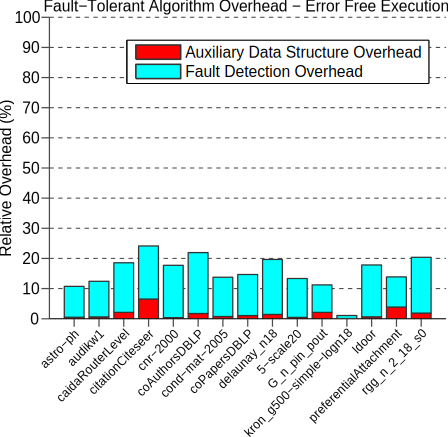
\includegraphics[height=.75\textheight]{plots/plot_zero_overhead-1}

\color{dpg} On an average 1.3\% overhead for maintaining additional data structure and 14\%
for fault detection.
\lyxframeend{}

%%%%%%%%%%%%%%%%%%%%%%%%%%%%%%%%%%%%%%%%%%%%%%%%%%%%%%%%%
\lyxframe{Failure Rate for synchronous case }
\centering
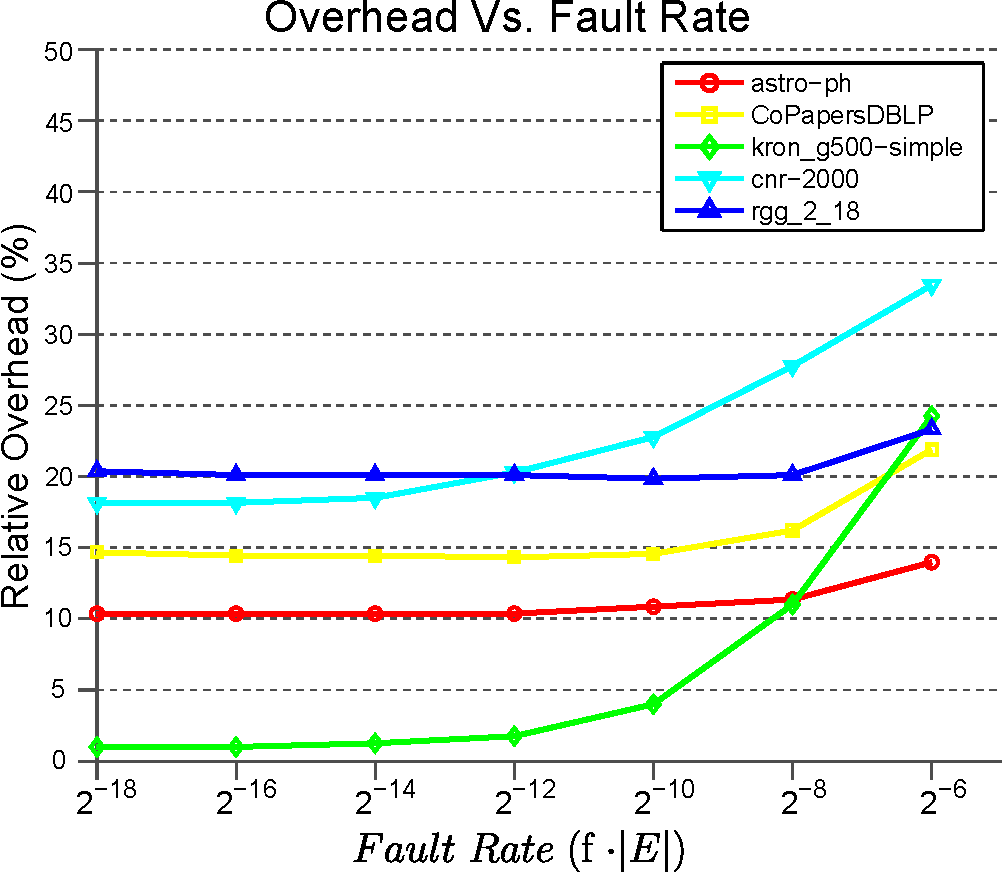
\includegraphics[height=.75\textheight]{plots/plot_overhead_fault-inked}

\lyxframeend{}
%%%%%%%%%%%%%%%%%%%%%%%%%%%%%%%%%%%%%%%%%%%%%%%%%%%%%%%%%


%%%%%%%%%%%%%%%%%%%%%%%%%%%%%%%%%%%%%%%%%%%%%%%%%%%%%%%%%
\lyxframe{Fault free overhead }
\centering
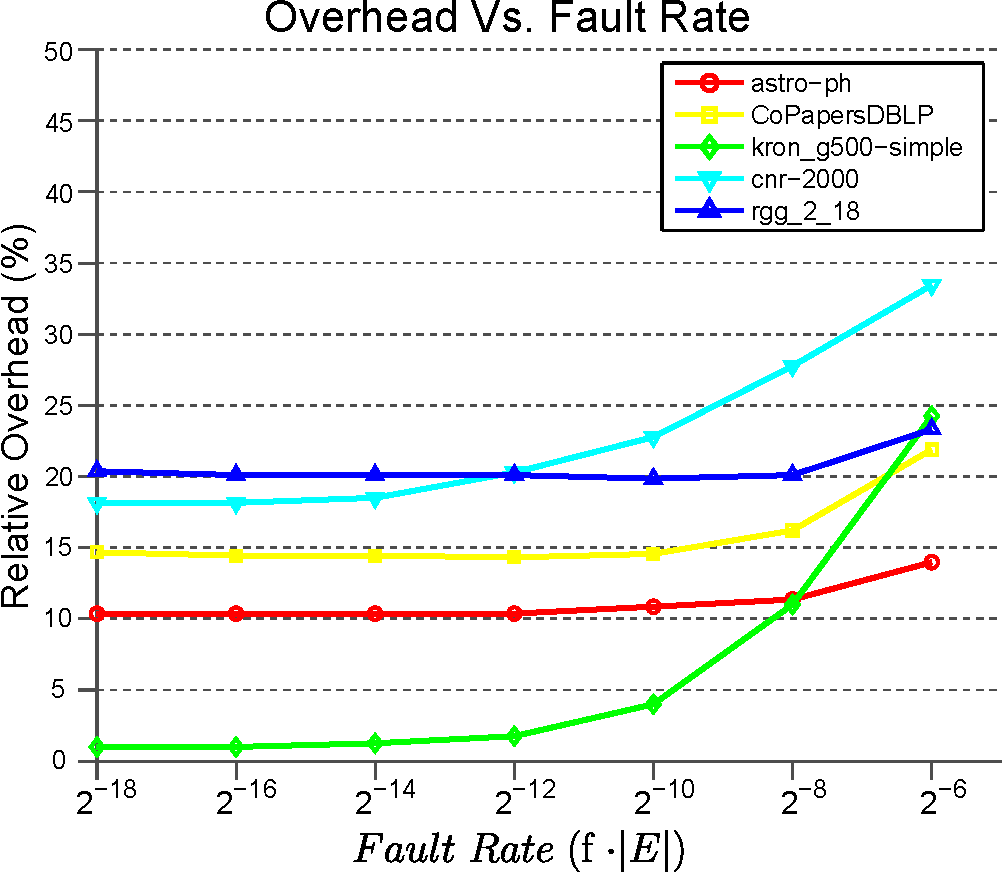
\includegraphics[height=.75\textheight]{plots/plot_overhead_fault-inked}

\lyxframeend{}
%%%%%%%%%%%%%%%%%%%%%%%%%%%%%%%%%%%%%%%%%%%%%%%%%%%%%%%%%

%%%%%%%%%%%%%%%%%%%%%%%%%%%%%%%%%%%%%%%%%%%%%%%%%%%%%%%%%
\lyxframe{Failure Rate for asynchronous case }
\centering
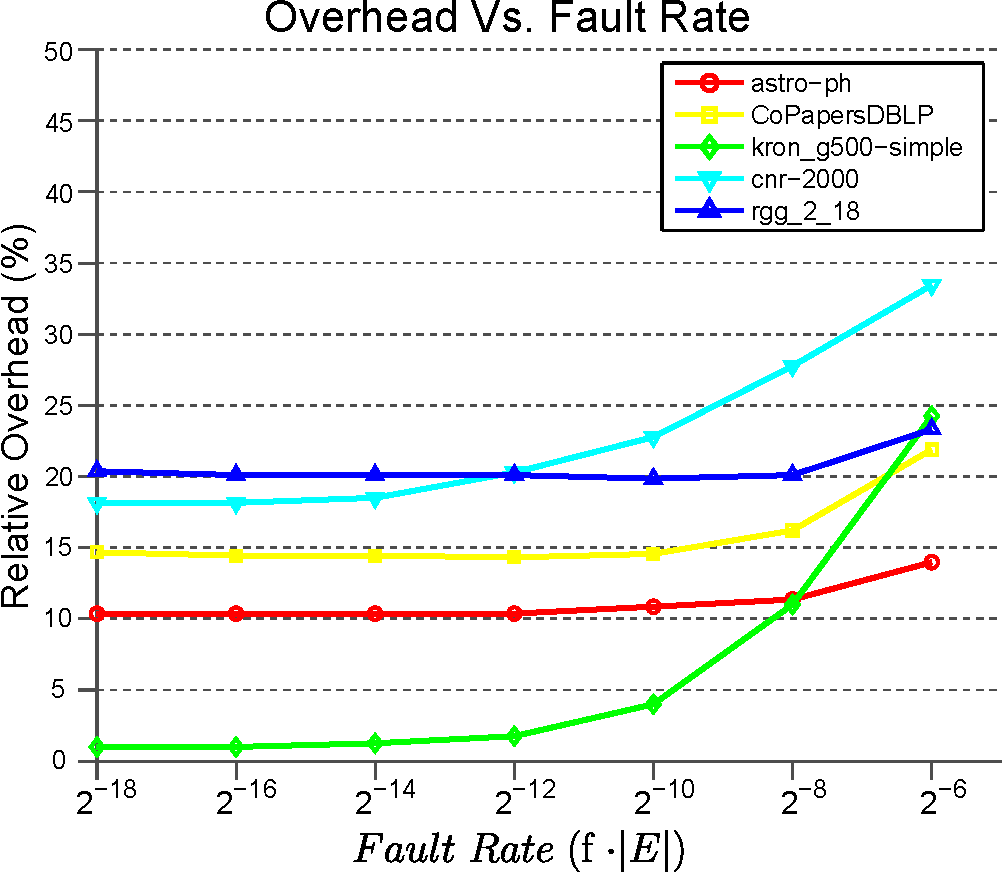
\includegraphics[height=.75\textheight]{plots/plot_overhead_fault-inked}

\lyxframeend{}
%%%%%%%%%%%%%%%%%%%%%%%%%%%%%%%%%%%%%%%%%%%%%%%%%%%%%%%%%


%%%%%%%%%%%%%%%%%%%%%%%%%%%%%%%%%%%%%%%%%%%%%%%%%%%%%%%%%
\lyxframe{Histogram for convergence}
\centering
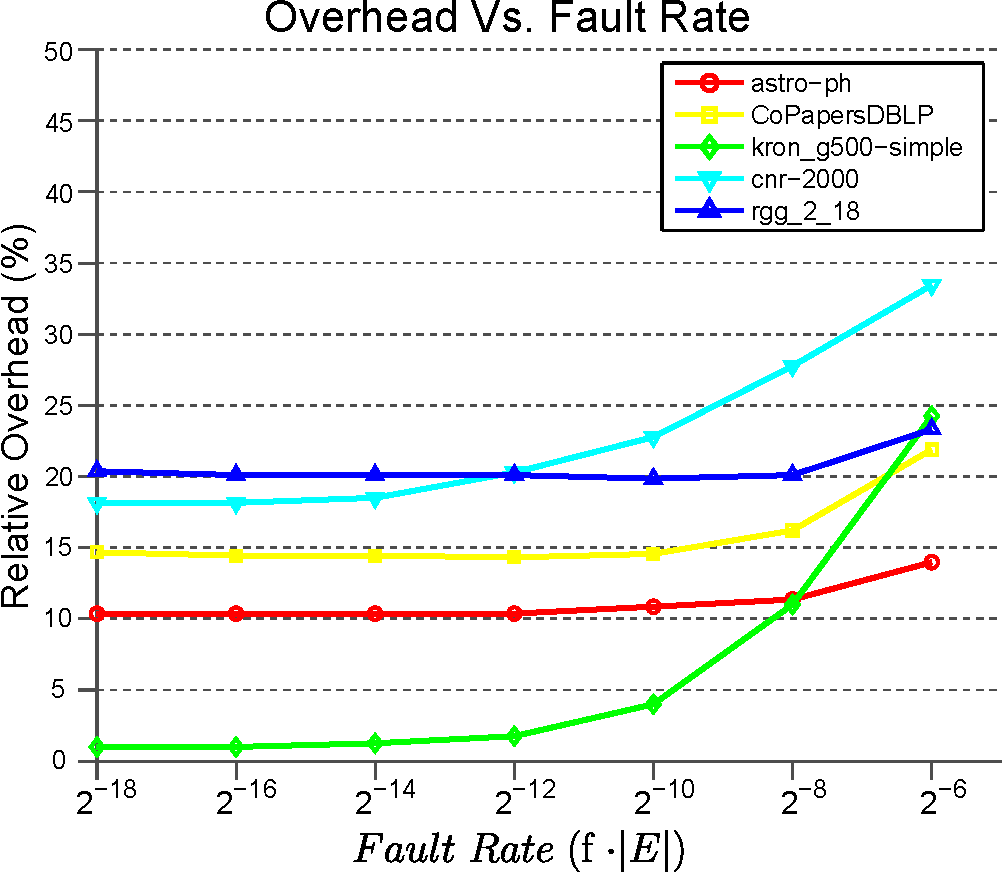
\includegraphics[height=.75\textheight]{plots/plot_overhead_fault-inked}
\lyxframeend{}
%%%%%%%%%%%%%%%%%%%%%%%%%%%%%%%%%%%%%%%%%%%%%%%%%%%%%%%%%




\section{Related work}
\label{sec:related}
Here goes the related work \cite{shantharam2012fault}.

\section{Conclusion and Future Work}
\label{sec:conclusion} \textbf{\emph{c}}\emph{onlusion} 
\begin{itemize}
\item what did we do 
\item what are implications 
\item where do we go from here 
\end{itemize}



% \subsection*{Acknowledgments}

% \input{ack}

\bibliographystyle{ieeetr}
\bibliography{sao} 

\end{document}
